\chapter{Studied systems}
\todoa{Write about the systems we studied}%
\todoa{Rename flat fracture systems to reference?}
\todoa{Write about density and vacuum problems}
%
% flat_square_fracture02
% flat_square_fracture03
% flat_fracture02
% flat_fracture03
% rough_fracture01_abel
% rough_fracture03
% rough_fracture04_same_distance
% rough_fracture05
%
We have do experiments on a total of 8 different systems, all consisting of a slab of silica with a fracture in the center filled with water. Four of them are ``reference'' systems with just a flat fracture in the center, and the other four are systems with a random fracture with different geometries.

All systems are created using the experimental procedure from \cref{sec:experimental_procedure}. The systems are initialized as a perfect crystal of $\upbeta$-cristobalite. The system is then brought to 4500 Kelvin using a thermostat, to melt the silica crystal. It is then cooled back down to 300 Kelvin, and a fracture is cut out of the solid slab of silica, the system dangling ends are passivated, and the fracture is filled with water. The system is then thermalized at 300 Kelvin.

A summary of the different systems can be seen in \cref{tab:systems}, where we have listed the dimension, porosity, the number of atoms, and the number of SiO$_2$ and water \hl{units/species} in each system.

The fractures in the systems labelled ``rough fracture'' are all created using periodic surfaces with a Hurst exponent close to \hl{0.75}, generated using successive random additions from \cref{sec:diamond_square_2d_finite}, and the fractures cut out using the method from \cref{sec:generating_fractures}. Systems 1 and 2 are created using different surfaces for the top and bottom of the fracture, while system 3 and 4 are created using the same surface repeated twice for the top and bottom of the fracture, with a distance of respectively 14.4 and 28.8 \AA\ between the surfaces.

\begin{table}[htpb]
\centering
    \begin{tabular}{l|cccccc}
    \textit{System}             & \textit{Dimensions} [\AA]     & $\phi$ [\%]   & \textit{r} [\AA]  & $N$       & $N_\text{SiO$_2$}$    & $N_\text{H$_2$O}$ \\ \hline 
    Flat fracture \#1           & $179 \times 179 \times 179$   & 48            & 86                & 260 k     & 25 k                  & 60 k                             \\ % flat_square_fracture02, N = 259955
    Flat fracture \#2           & $179 \times 179 \times 179$   & 48            & 86                & 271 k     & 25 k                  & 64 k                             \\ % flat_square_fracture03, N = 271328
    Flat fracture \#3           & $143 \times 143 \times 57$    & 25            & 14.4              & 90 k      & 19 k                  & 10 k                             \\ % flat_fracture02, N = 89646
    Flat fracture \#4           & $143 \times 143 \times 57$    & 50            & 28.8              & 107 k     & 13 k                  & 22 k                             \\ % flat_fracture03, N = 106829
    \hline %
    Rough fracture \#1          & $179 \times 179 \times 179$   & ${\sim}12$    & -                 & 393 k  & 111 k                    & 19 k           \\ % rough_fracture01_abel, N = 393181
    Rough fracture \#2          & $172 \times 172 \times 172$   & ${\sim}13$    & -                 & 347 k  & 97 k                     & 18 k            \\ %rough_fracture03, N = 347176
    Rough fracture \#3          & $172 \times 172 \times 172$   & ${\sim}13$    & 14.4              & 349 k  & 99 k                     & 16 k            \\ % rough_fracture04_same_distance, N = 348573
    Rough fracture \#4          & $172 \times 172 \times 172$   & ${\sim}23$    & 28.8              & 368 k  & 89 k                     & 34 k            \\ % rough_fracture05 N = 367958
    \end{tabular}%
    \vspace{8pt}
    \caption{%
%     \caption{%
%     a
        An overview of the 8 different systems we have done experiments on. ``Flat fracture'' 1 through 4 are reference systems, that consist of a silica slab with a single flat fracture filled with water. ``Rough fracture'' 1 through 4 consist of a silica slab with different water-filled fractures with different geometries.%
        \\%
%
        $\phi$ is the approximate porosity of the system, defined as the volume of the fracture relative to the volume of the whole system. $r$ is the distance between the surfaces used to create the fracture. $N$ is the total number of atoms (silicon, oxygen and hydrogen), $N_\text{SiO$_2$}$ is the number of SiO$_2$-units, and $N_\text{H$_2$O}$ is the number of water molecules. %
%
%         $N_\text{H$_2$O}$ and $N_\text{SiO$_2$}$ measured in flat02 and flat03 using slice of heigth 14.4/28.8, and then counting number of oxygen/silicon in slice. \hl{Volumes of rough fractures calculated using Ovito ``construct surface mesh''}%
        \label{tab:systems}%
%     }%
    }
\end{table}%

\FloatBarrier
\section{Visualizations}
We have made some renderings of the systems we have studied, as can be seen in \crefrange{fig:renderings_rough_fracture01_abel}{fig:renderings_flat_fractures}\todoao{Check that this range is correct before handing in}. All renderings and visualizations were made using the program Ovito\cite{stukowski2010ovito}, using the built-in open-source ``Tachyon'' rendering engine.

In the renderings in this section we have colored the silicon atoms yellow, the oxygen atoms blue, and the hydrogen atoms white. The silicon atoms have been given a radius of 1 \AA, the oxygen atoms 0.6 \AA, and the hydrogen atoms 0.3 \AA.
%
\begin{figure}[!p]%
    \centering%
    \setlength{\myfigwidth}{0.49\textwidth}%
%     \setlength{\mycaptionwidth}{0.3\textwidth}%
%
    \begin{subfigure}[t]{\myfigwidth}%
        \centering% % Need to center to get image centered over caption
        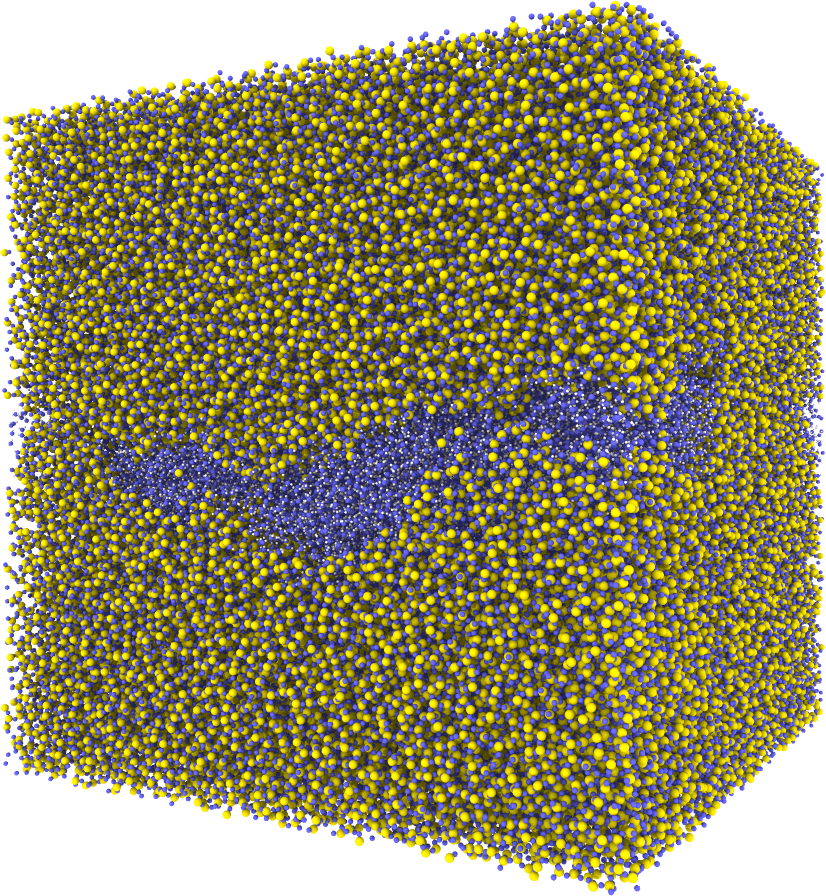
\includegraphics[width=\textwidth]{images/systems/trimmed-rough_fracture01_abel_13}%
        \caption{The whole system.}%
%         \label{fig:hex_to_tetra}%
    \end{subfigure}%
    \hfill%
        \begin{subfigure}[t]{\myfigwidth}%
        \centering% % Need to center to get image centered over caption
        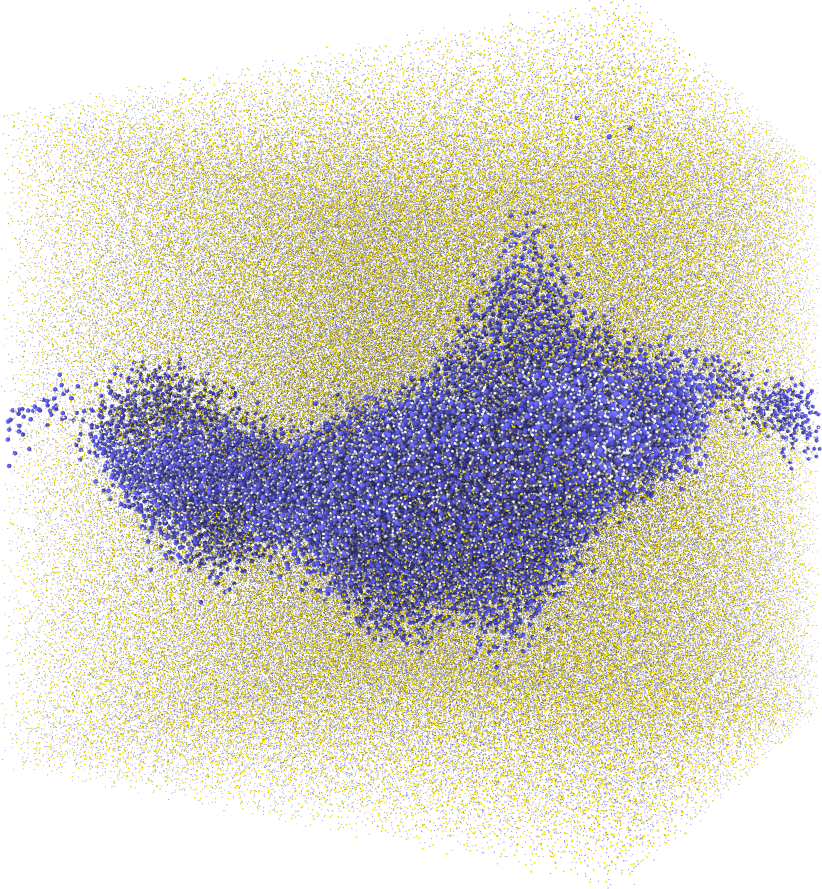
\includegraphics[width=\textwidth]{images/systems/trimmed-rough_fracture01_abel_15}%
        \caption{The whole system, with the size of the silicon and silica-oxygen atoms reduced to 0.1 \AA.}%
%         \label{fig:hex_to_tetra}%
    \end{subfigure}%
    \vspace{10pt}\\%
    \begin{subfigure}[t]{\myfigwidth}%
        \centering% % Need to center to get image centered over caption
        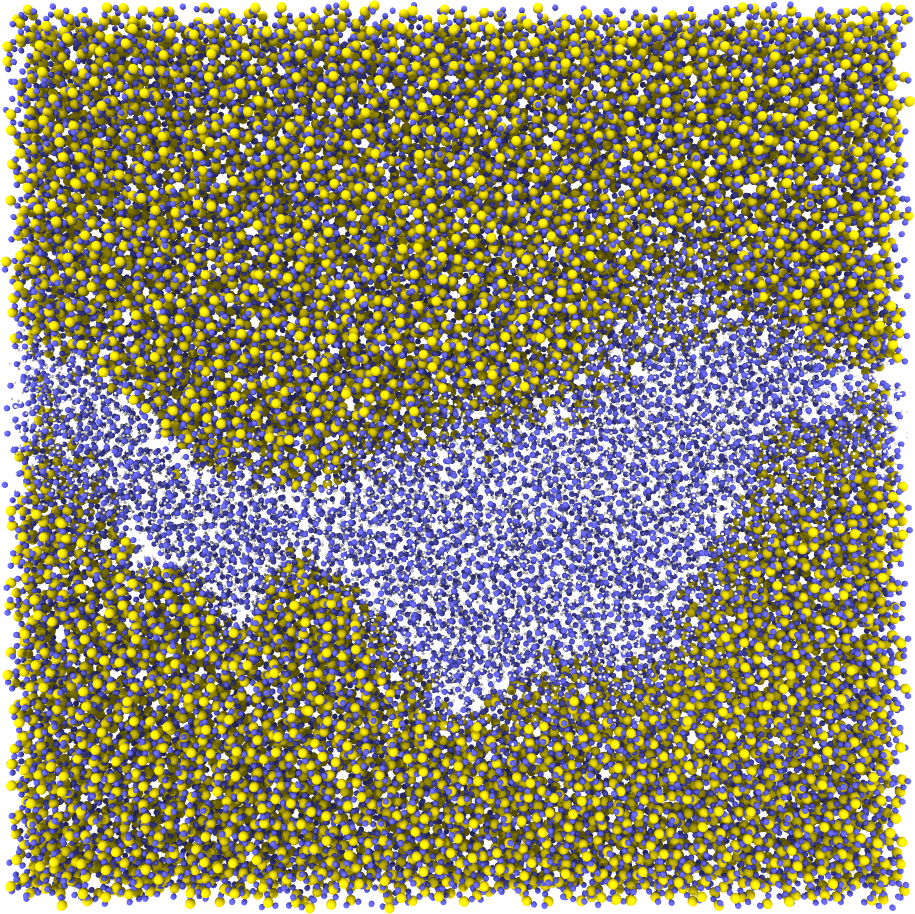
\includegraphics[width=\textwidth]{images/systems/trimmed-rough_fracture01_abel_16}%
        \caption{20 \AA\ thick slice.}%
%         \label{fig:hex_to_tetra}%
    \end{subfigure}%
    \hfill%
    %
    % ---- Rendering just water atoms ---- %
%     \begin{subfigure}[t]{\myfigwidth}%
%         \centering% % Need to center to get image centered over caption
%         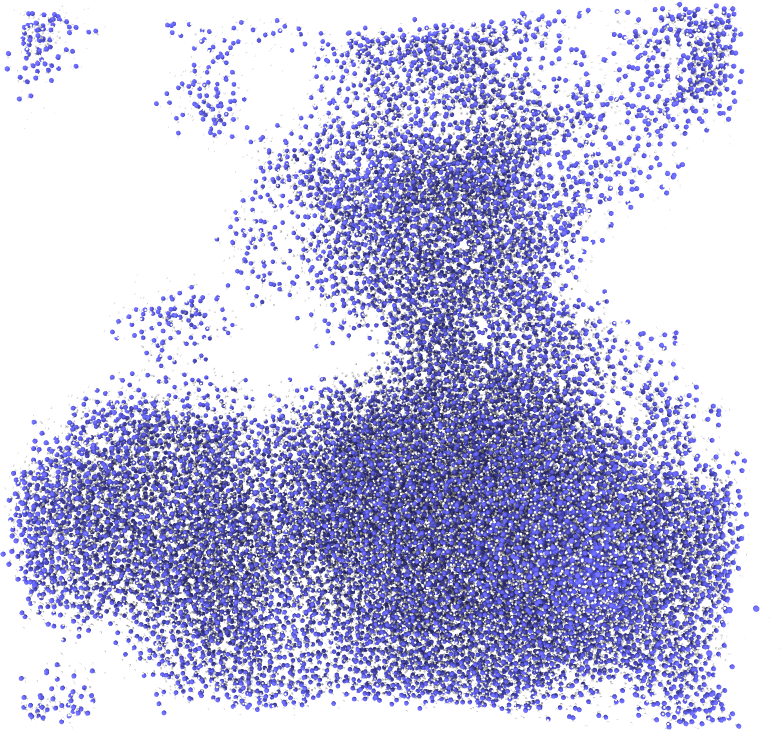
\includegraphics[width=\textwidth]{images/systems/trimmed-rough_fracture01_abel_17}%
%         \caption{Just the water molecules, viewed from above.}%
% %         \label{fig:hex_to_tetra}%
%     \end{subfigure}%
    % ----
    %
    % ---- Rendering of the water volume ---- %
    \begin{subfigure}[t]{\myfigwidth}%
        \centering% % Need to center to get image centered over caption
        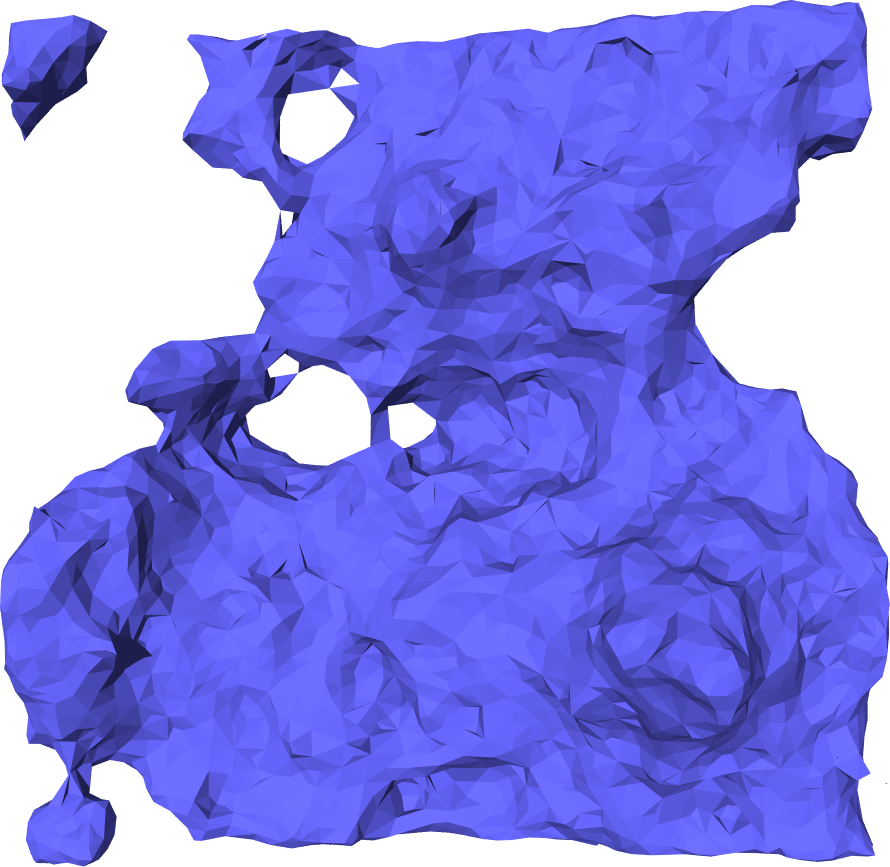
\includegraphics[width=\textwidth]{images/systems/trimmed-rough_fracture01_abel_22}%
        \caption{The pore volume.}%
%         \label{fig:hex_to_tetra}%
    \end{subfigure}%
    % ----
    \vspace{10pt}\\%
    \caption{%
        ``Rough fracture \#1'', a randomly generated fracture with varying width. \hl{Caption} %
        \label{fig:renderings_rough_fracture01_abel}%
    }%
\end{figure}%

%
\begin{figure}[!p]%
    \centering%
    \setlength{\myfigwidth}{0.55\textwidth}%
    \setlength{\myhfillwidth}{5mm}%
%     \setlength{\mycaptionwidth}{0.3\textwidth}%
%
% Use makebox to center figures below that are wider than \textwidth
%
\makebox[\textwidth][c]{%
    \begin{subfigure}[t]{\myfigwidth}%
        \centering% % Need to center to get image centered over caption
        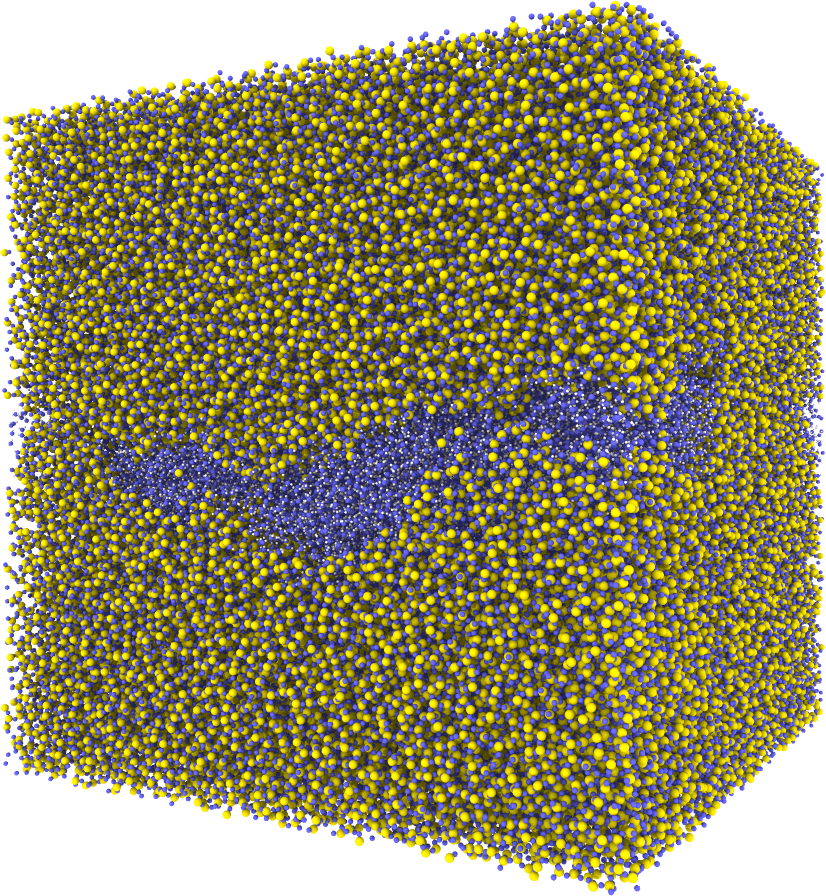
\includegraphics[width=\textwidth]{images/systems/trimmed-rough_fracture01_abel_13}%
        \caption{The whole system.}%
%         \label{fig:hex_to_tetra}%
    \end{subfigure}%
    %\hfill%
    \hspace{\myhfillwidth}%
        \begin{subfigure}[t]{\myfigwidth}%
        \centering% % Need to center to get image centered over caption
        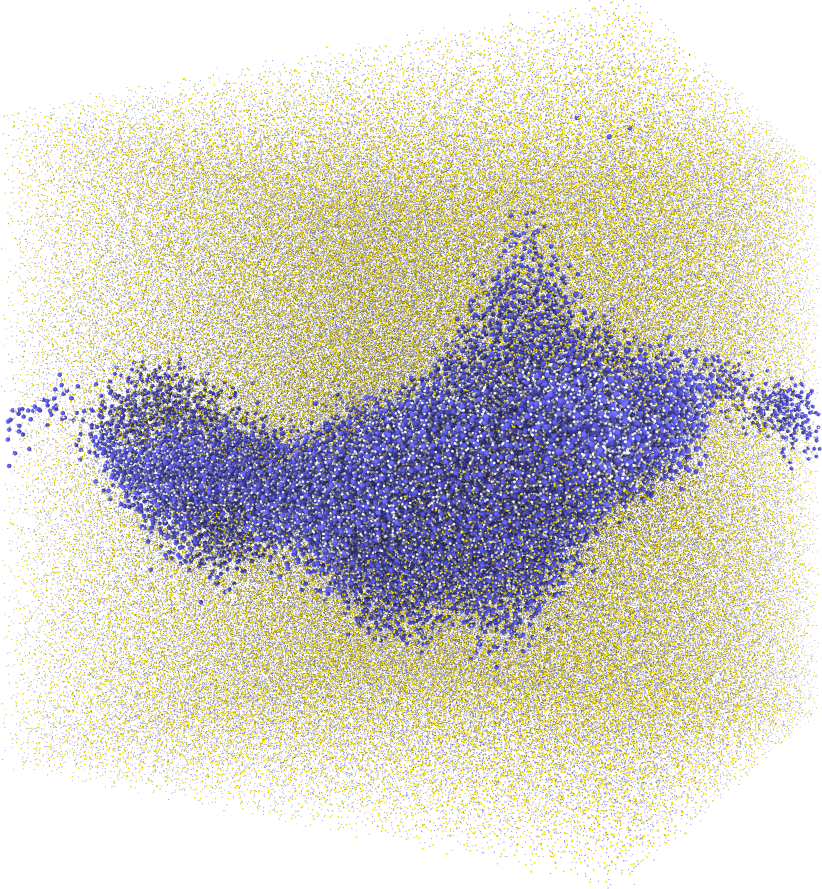
\includegraphics[width=\textwidth]{images/systems/trimmed-rough_fracture01_abel_15}%
        \caption{The whole system, with the size of the silicon and silica-oxygen atoms reduced to 0.1 \AA.}%
%         \label{fig:hex_to_tetra}%
    \end{subfigure}%
}%
    \vspace{10pt}\\%
\makebox[\textwidth][c]{%
    \begin{subfigure}[t]{\myfigwidth}%
        \centering% % Need to center to get image centered over caption
        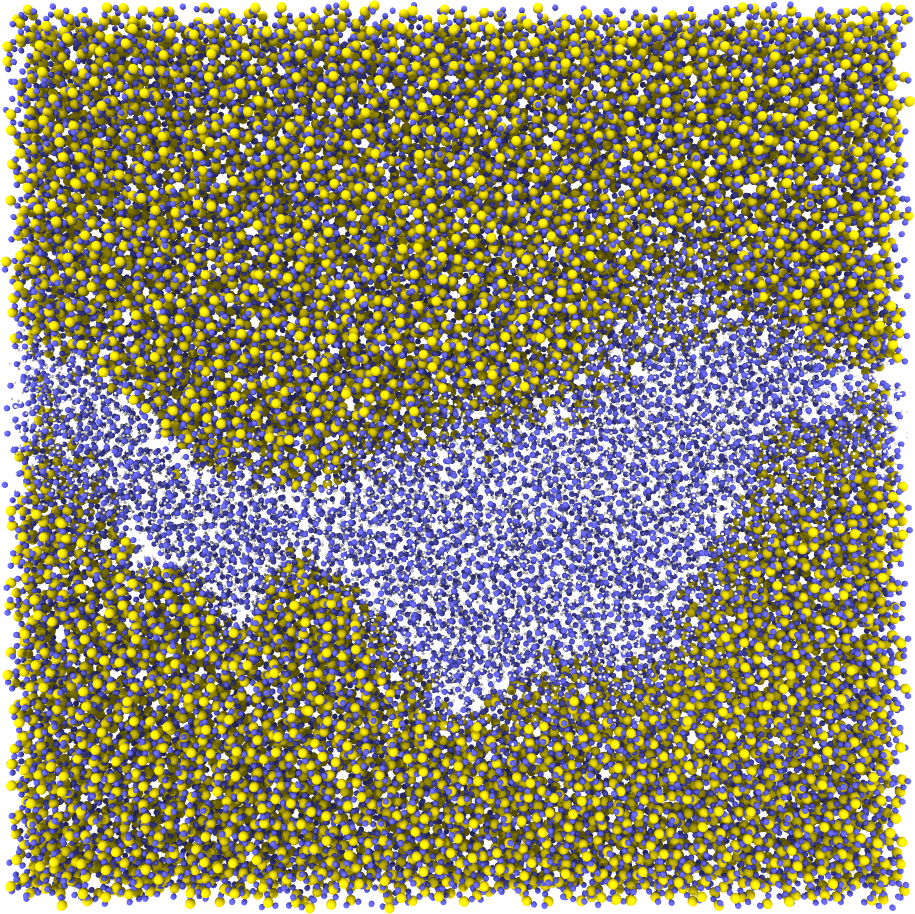
\includegraphics[width=\textwidth]{images/systems/trimmed-rough_fracture01_abel_16}%
        \caption{20 \AA\ thick slice.}%
%         \label{fig:hex_to_tetra}%
    \end{subfigure}%
%     \hfill%
    \hspace{\myhfillwidth}%
    %
    % ---- Rendering just water atoms ---- %
%     \begin{subfigure}[t]{\myfigwidth}%
%         \centering% % Need to center to get image centered over caption
%         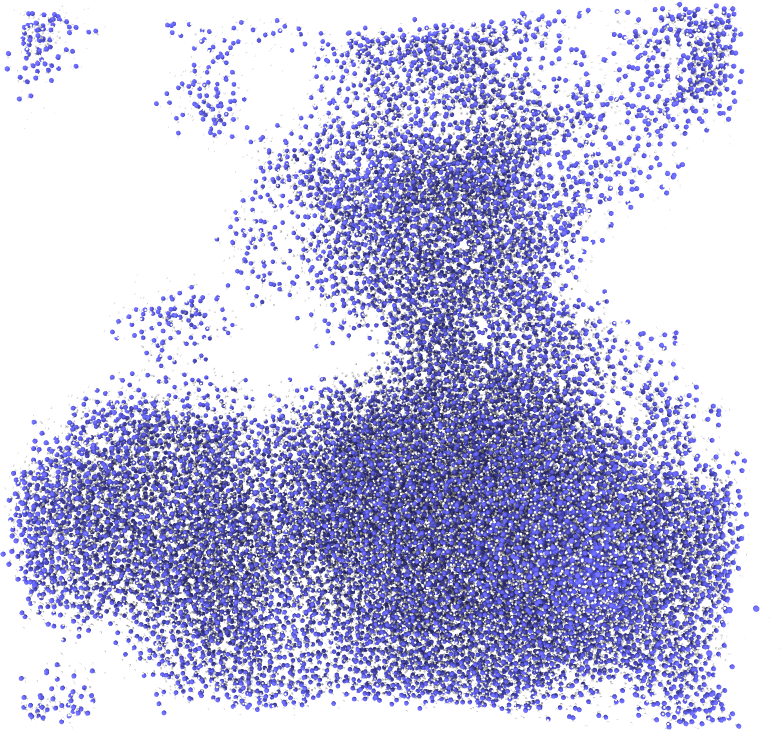
\includegraphics[width=\textwidth]{images/systems/trimmed-rough_fracture01_abel_17}%
%         \caption{Just the water molecules, viewed from above.}%
% %         \label{fig:hex_to_tetra}%
%     \end{subfigure}%
    % ----
    %
    % ---- Rendering of the water volume ---- %
    \begin{subfigure}[t]{\myfigwidth}%
        \centering% % Need to center to get image centered over caption
        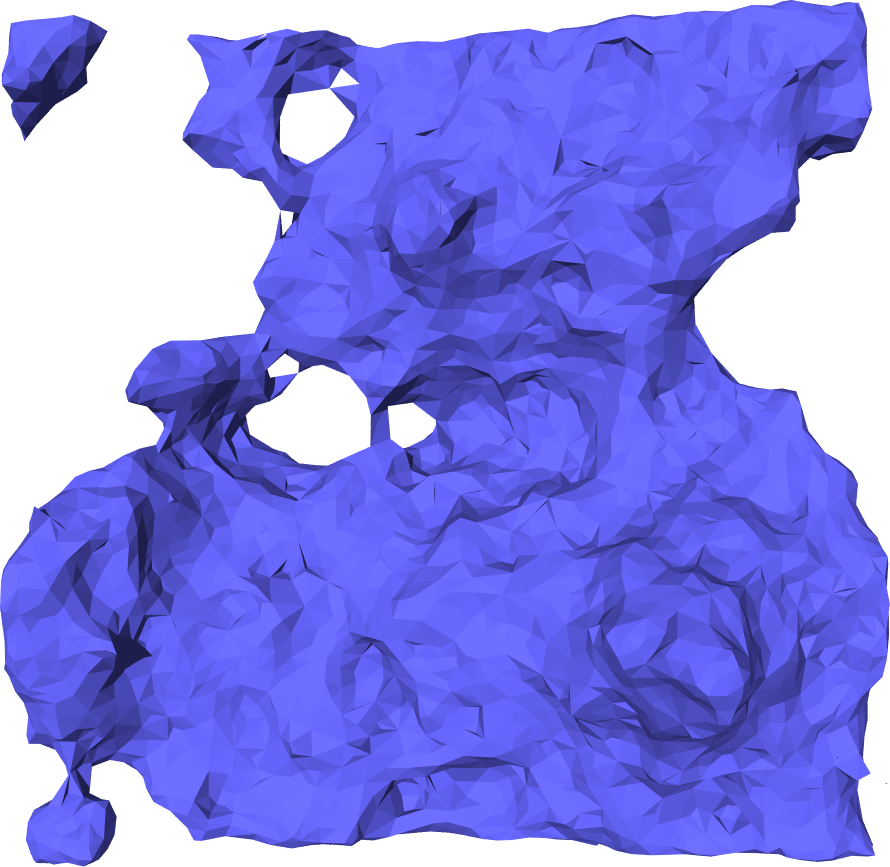
\includegraphics[width=\textwidth]{images/systems/trimmed-rough_fracture01_abel_22}%
        \caption{The pore volume.}%
%         \label{fig:hex_to_tetra}%
    \end{subfigure}%
    % ----
}%
    \vspace{10pt}\\%
    \caption{%
        ``Rough fracture \#1'', a randomly generated fracture with varying width. \hl{Caption} %
        \label{fig:renderings_rough_fracture01_abel}%
    }%
\end{figure}%

%
\begin{figure}[!p]%
    \centering%
    \setlength{\myfigwidth}{0.49\textwidth}%
%     \setlength{\mycaptionwidth}{0.3\textwidth}%
%
    \begin{subfigure}[t]{\myfigwidth}%
        \centering% % Need to center to get image centered over caption
        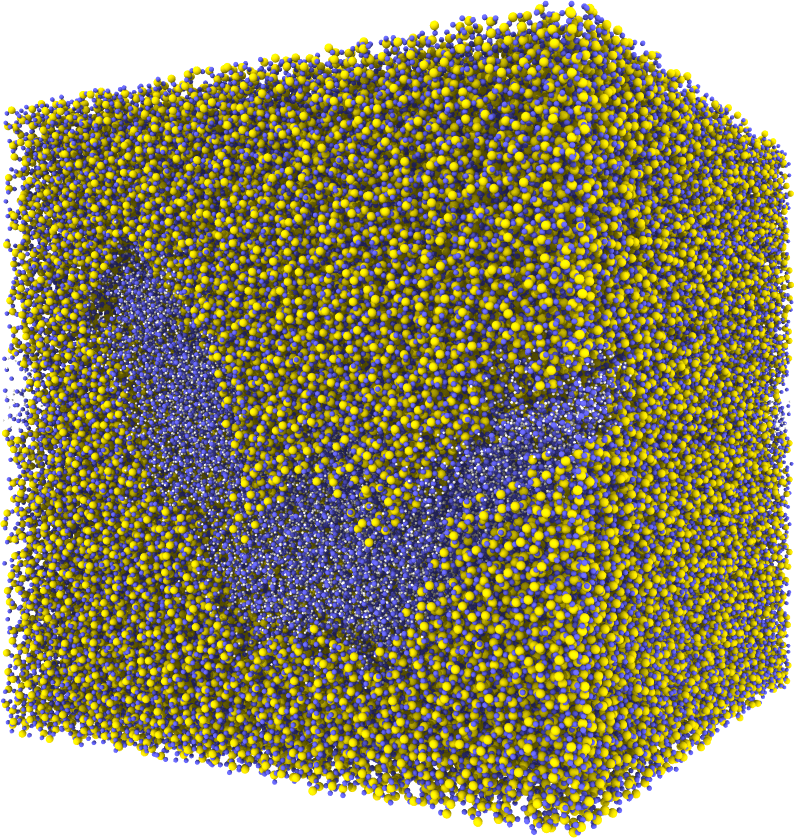
\includegraphics[width=\textwidth]{images/systems/trimmed-rough_fracture03_06}%
        \caption{The whole system.}%
%         \label{fig:hex_to_tetra}%
    \end{subfigure}%
    \hfill%
    \begin{subfigure}[t]{\myfigwidth}%
        \centering% % Need to center to get image centered over caption
        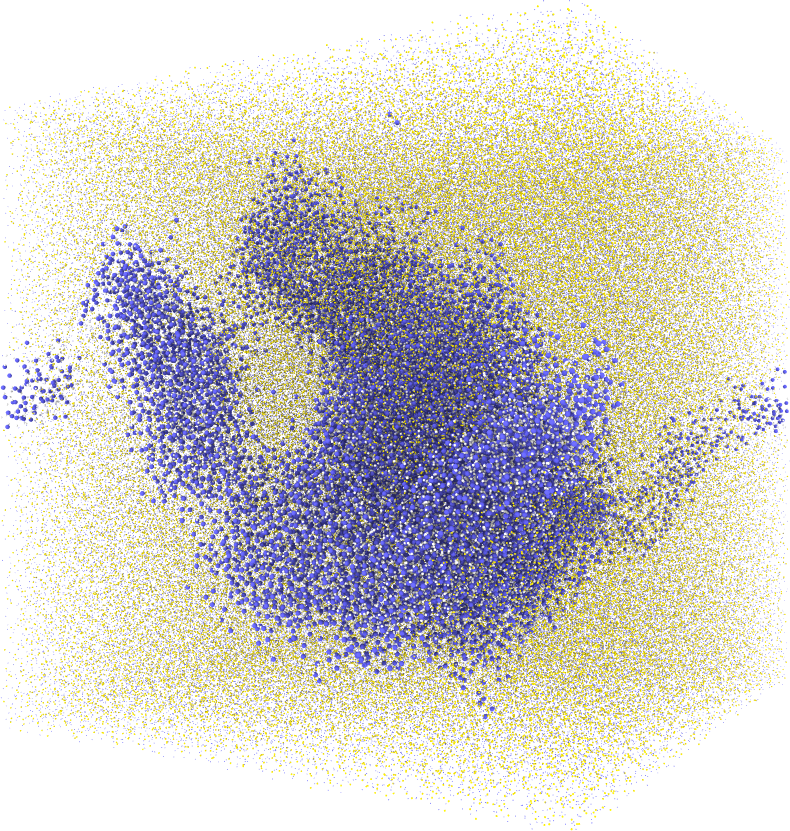
\includegraphics[width=\textwidth]{images/systems/trimmed-rough_fracture03_05}%
        \caption{The whole system, with the size of the silicon and silica-oxygen atoms reduced to 0.1 \AA.}%
%         \label{fig:hex_to_tetra}%
    \end{subfigure}%
    \vspace{10pt}\\%
    \begin{subfigure}[t]{\myfigwidth}%
        \centering% % Need to center to get image centered over caption
        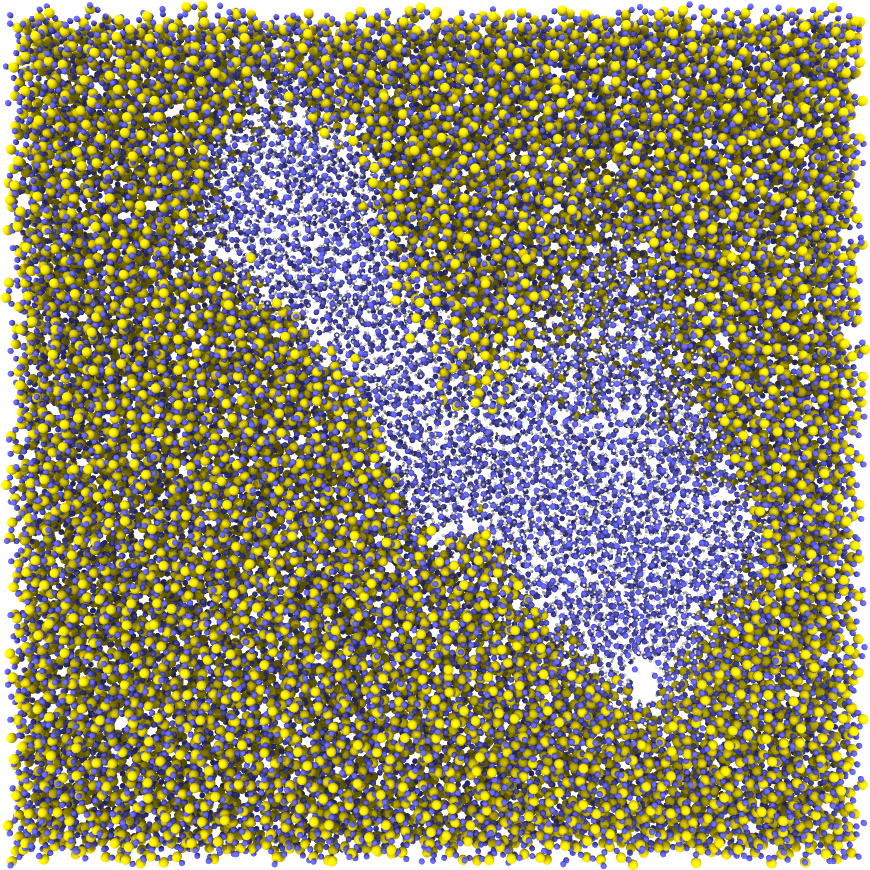
\includegraphics[width=\textwidth]{images/systems/trimmed-rough_fracture03_07}%
        \caption{20 \AA\ thick slice.}%
%         \label{fig:hex_to_tetra}%
    \end{subfigure}%
    \hfill%
    %
    % ---- Rendering just water atoms ---- %
%     \begin{subfigure}[t]{\myfigwidth}%
%         \centering% % Need to center to get image centered over caption
%         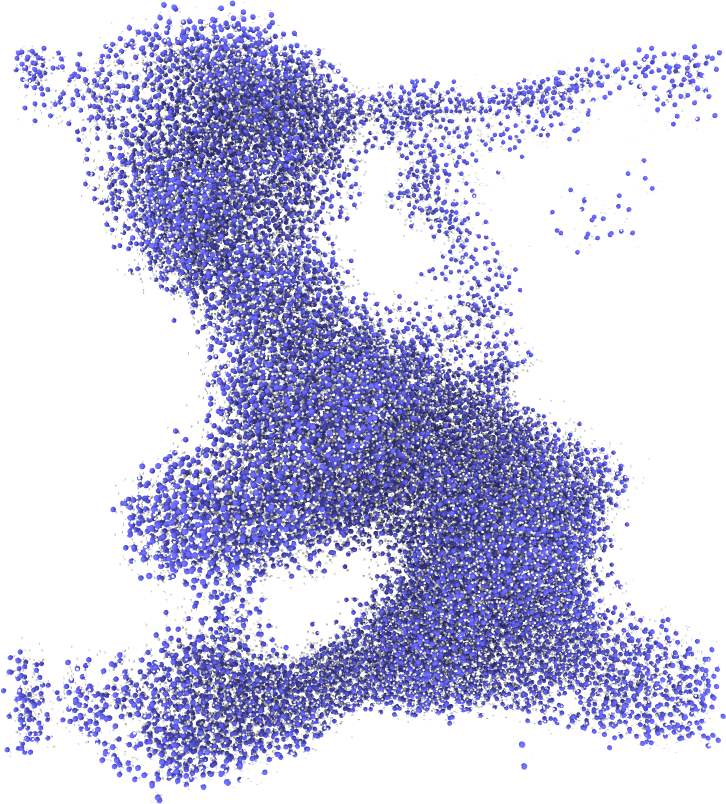
\includegraphics[width=\textwidth]{images/systems/trimmed-rough_fracture03_08}%
%         \caption{Caption.}%
% %         \label{fig:hex_to_tetra}%
%     \end{subfigure}%
    % ----
    %
    % ---- Rendering just water atoms ---- %
        \begin{subfigure}[t]{\myfigwidth}%
        \centering% % Need to center to get image centered over caption
        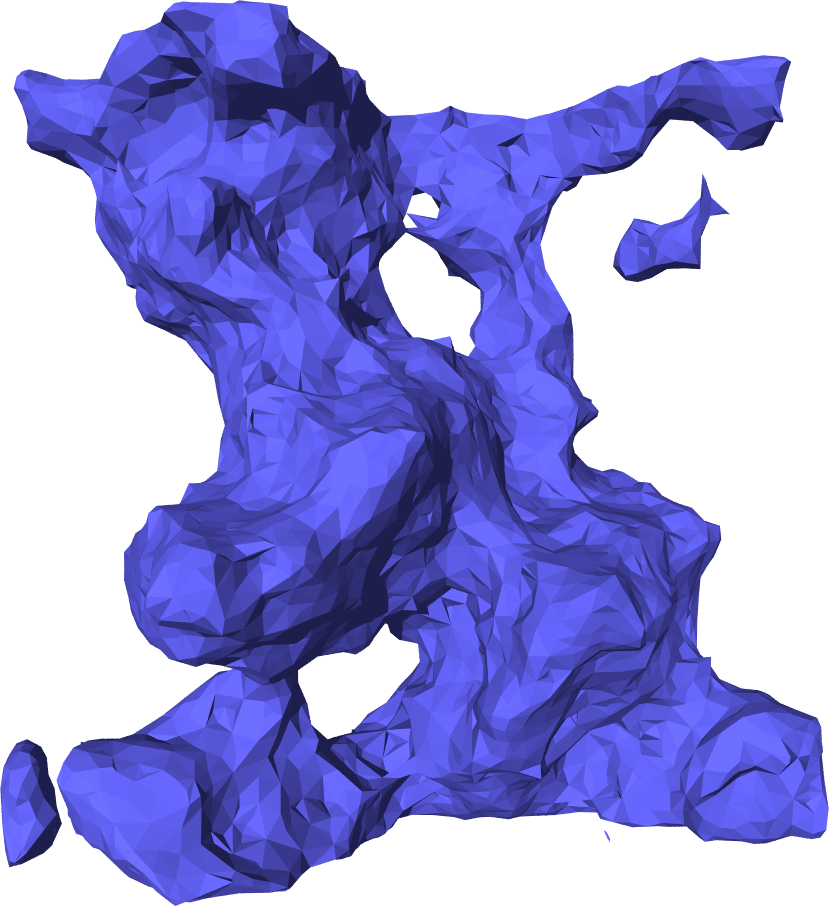
\includegraphics[width=\textwidth]{images/systems/trimmed-rough_fracture03_11}%
        \caption{The pore volume.}%
%         \label{fig:hex_to_tetra}%
    \end{subfigure}%
    % ----
    \vspace{10pt}\\%
    \caption{%
        ``Rough fracture \#2'', a randomly generated fracture with varying width. \hl{Caption} %
        \label{fig:renderings_rough_fracture03}%
    }%
\end{figure}%

%
\begin{figure}[!p]%
    \centering%
    \setlength{\myfigwidth}{0.49\textwidth}%
%     \setlength{\mycaptionwidth}{0.3\textwidth}%
%
    \begin{subfigure}[t]{\myfigwidth}%
        \centering% % Need to center to get image centered over caption
        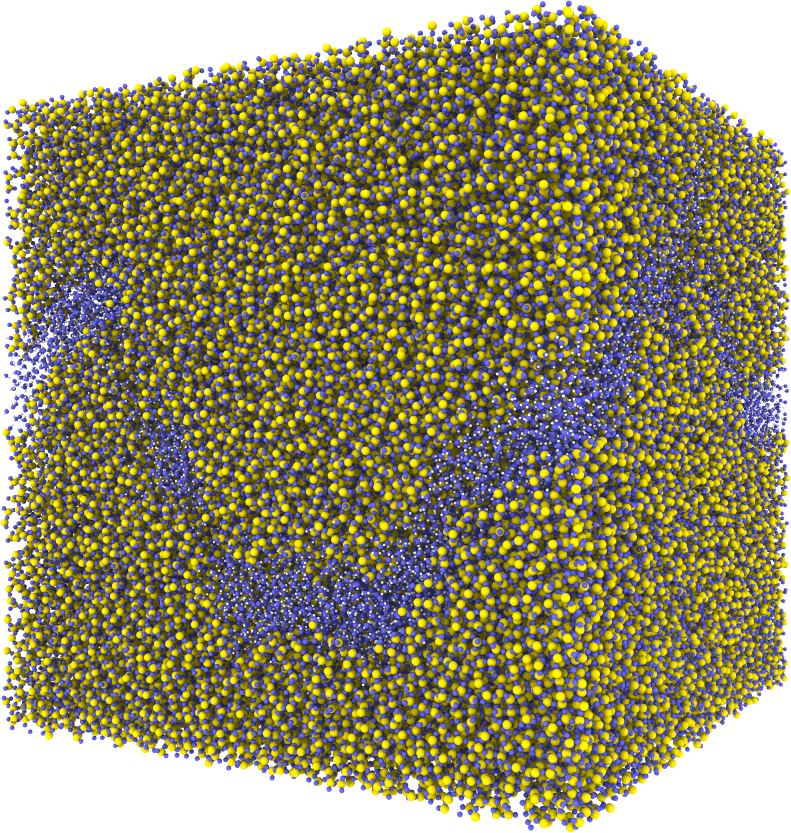
\includegraphics[width=\textwidth]{images/systems/trimmed-rough_fracture04_06}%
        \caption{The whole system.}%
%         \label{fig:hex_to_tetra}%
    \end{subfigure}%
    \hfill%
    \begin{subfigure}[t]{\myfigwidth}%
        \centering% % Need to center to get image centered over caption
        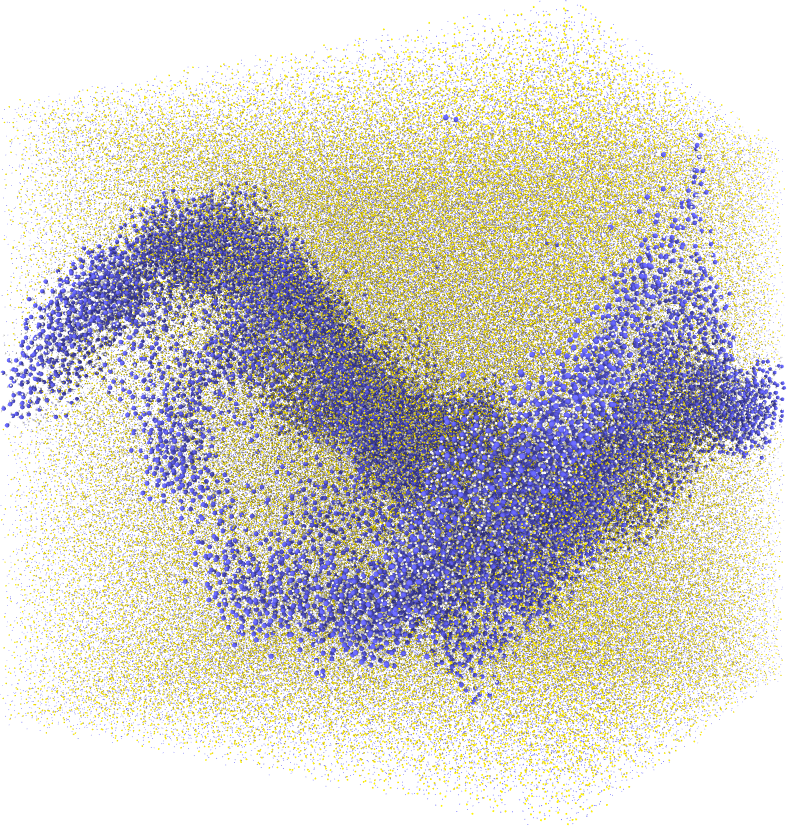
\includegraphics[width=\textwidth]{images/systems/trimmed-rough_fracture04_07}%
        \caption{The whole system, with the size of the silicon and silica-oxygen atoms reduced to 0.1 \AA.}%
%         \label{fig:hex_to_tetra}%
    \end{subfigure}%
    \vspace{10pt}\\%
    \begin{subfigure}[t]{\myfigwidth}%
        \centering% % Need to center to get image centered over caption
        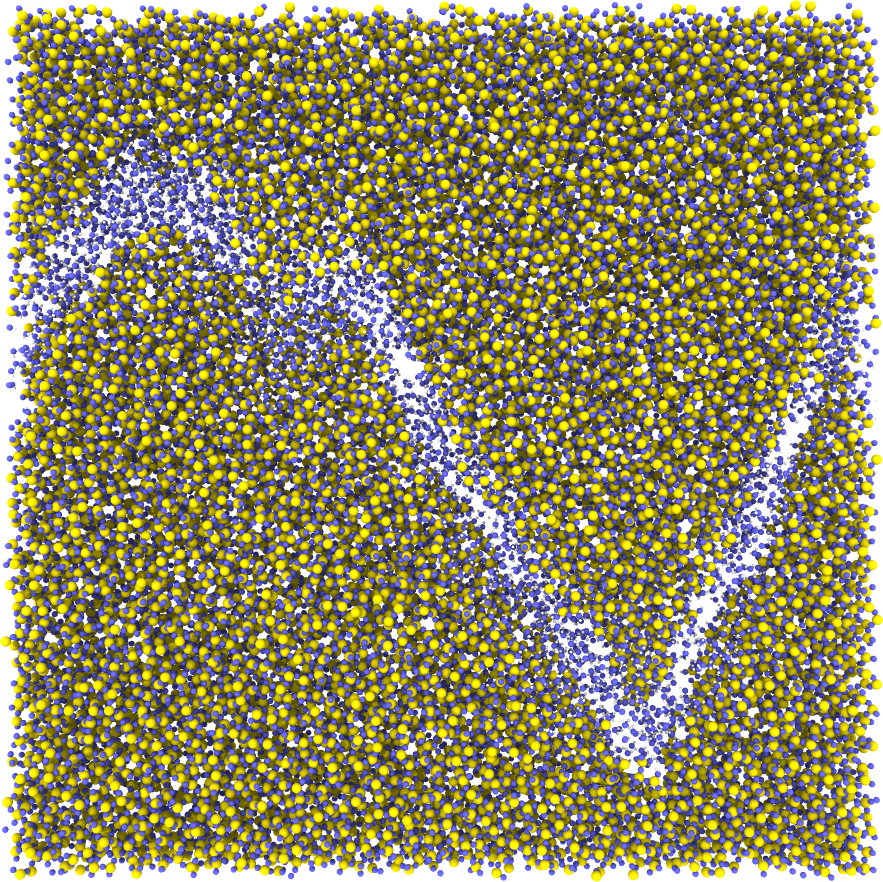
\includegraphics[width=\textwidth]{images/systems/trimmed-rough_fracture04_05_20ang}%
        \caption{20 \AA\ thick slice.}%
%         \label{fig:hex_to_tetra}%
    \end{subfigure}%
    \hfill%
    %
    % ---- Rendering just water atoms ---- %
%     \begin{subfigure}[t]{\myfigwidth}%
%         \centering% % Need to center to get image centered over caption
%         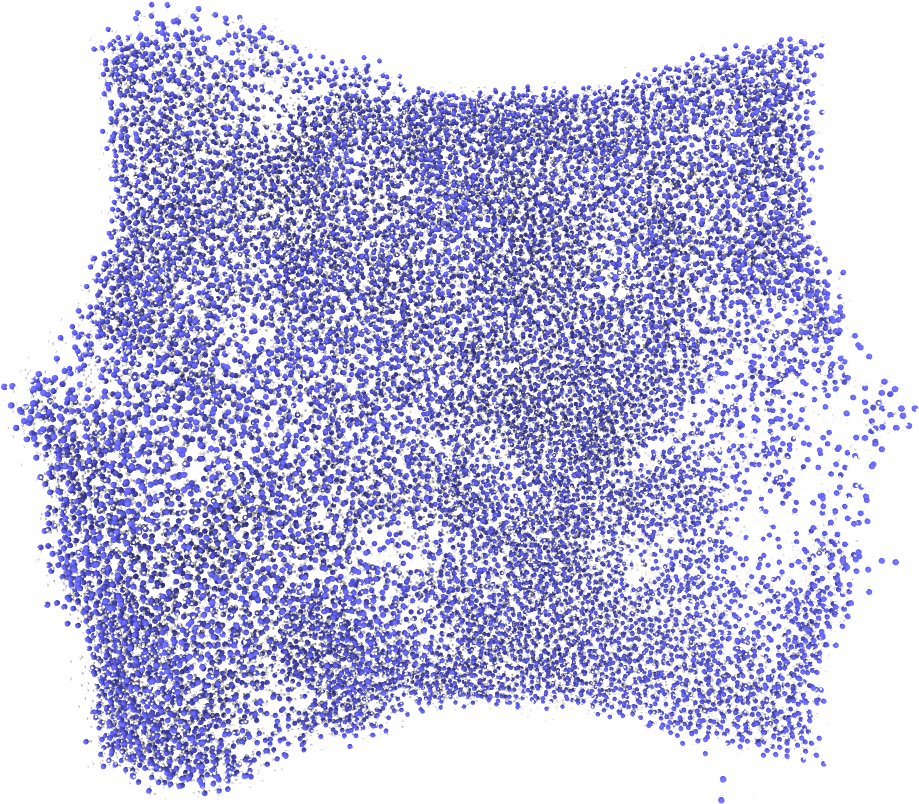
\includegraphics[width=\textwidth]{images/systems/trimmed-rough_fracture04_08}%
%         \caption{Caption.}%
% %         \label{fig:hex_to_tetra}%
%     \end{subfigure}%
    % ----
    %
    % ---- Rendering just water atoms ---- %
        \begin{subfigure}[t]{\myfigwidth}%
        \centering% % Need to center to get image centered over caption
        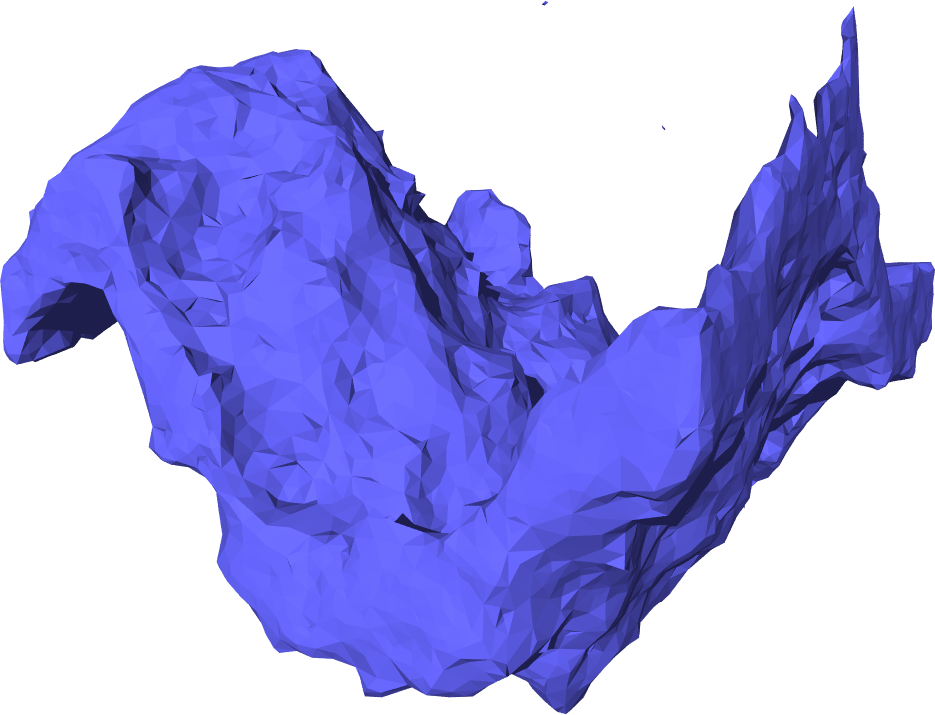
\includegraphics[width=\textwidth]{images/systems/trimmed-rough_fracture04_11}%
        \caption{The pore volume.}%
%         \label{fig:hex_to_tetra}%
    \end{subfigure}%
    % ----
    \vspace{10pt}\\%
    \caption{%
        ``Rough fracture \#3'', a randomly generated fracture generated from one surface repeated for the top and bottom half, with 14.4 \AA\ between the surfaces, giving approximately uniform width of the pore. \hl{Caption} %
        \label{fig:renderings_rough_fracture04_same_distance}%
    }%
\end{figure}%

%
\begin{figure}[!p]%
    \centering%
    \setlength{\myfigwidth}{0.49\textwidth}%
%     \setlength{\mycaptionwidth}{0.3\textwidth}%
%
    \begin{subfigure}[t]{\myfigwidth}%
        \centering% % Need to center to get image centered over caption
        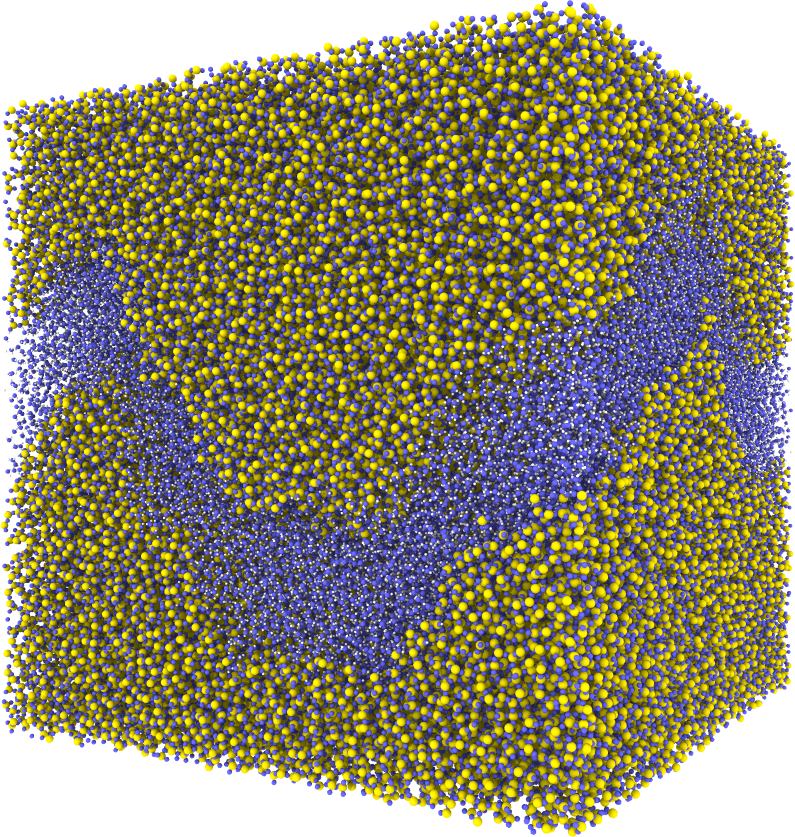
\includegraphics[width=\textwidth]{images/systems/trimmed-rough_fracture05_05}%
        \caption{The whole system.}%
%         \label{fig:hex_to_tetra}%
    \end{subfigure}%
    \hfill%
    \begin{subfigure}[t]{\myfigwidth}%
        \centering% % Need to center to get image centered over caption
        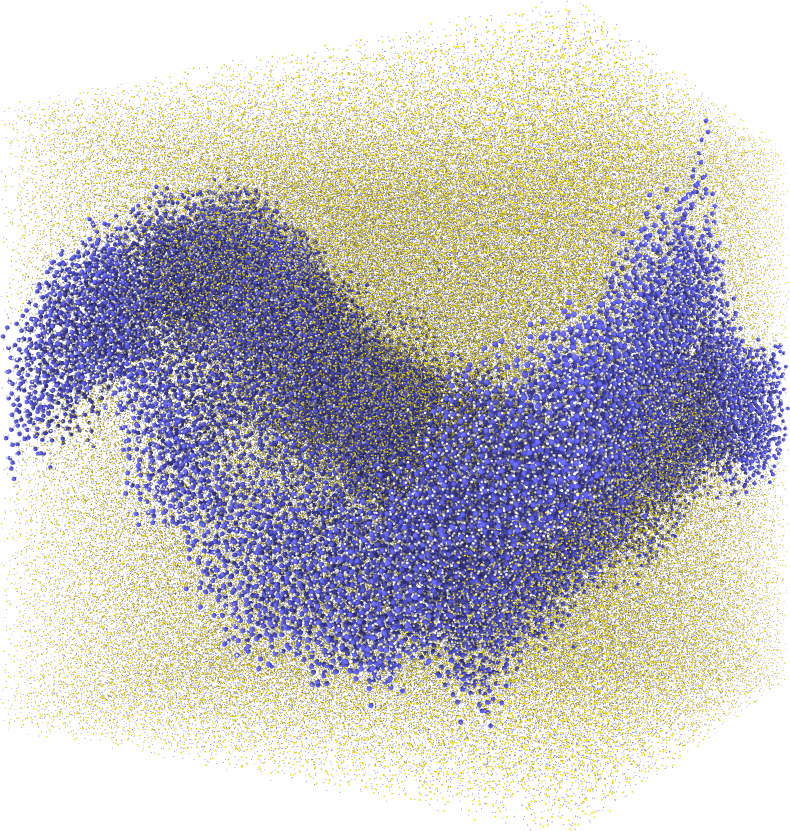
\includegraphics[width=\textwidth]{images/systems/trimmed-rough_fracture05_04}%
        \caption{The whole system, with the size of the silicon and silica-oxygen atoms reduced to 0.1 \AA.}%
%         \label{fig:hex_to_tetra}%
    \end{subfigure}%
    \vspace{10pt}\\%
    \begin{subfigure}[t]{\myfigwidth}%
        \centering% % Need to center to get image centered over caption
        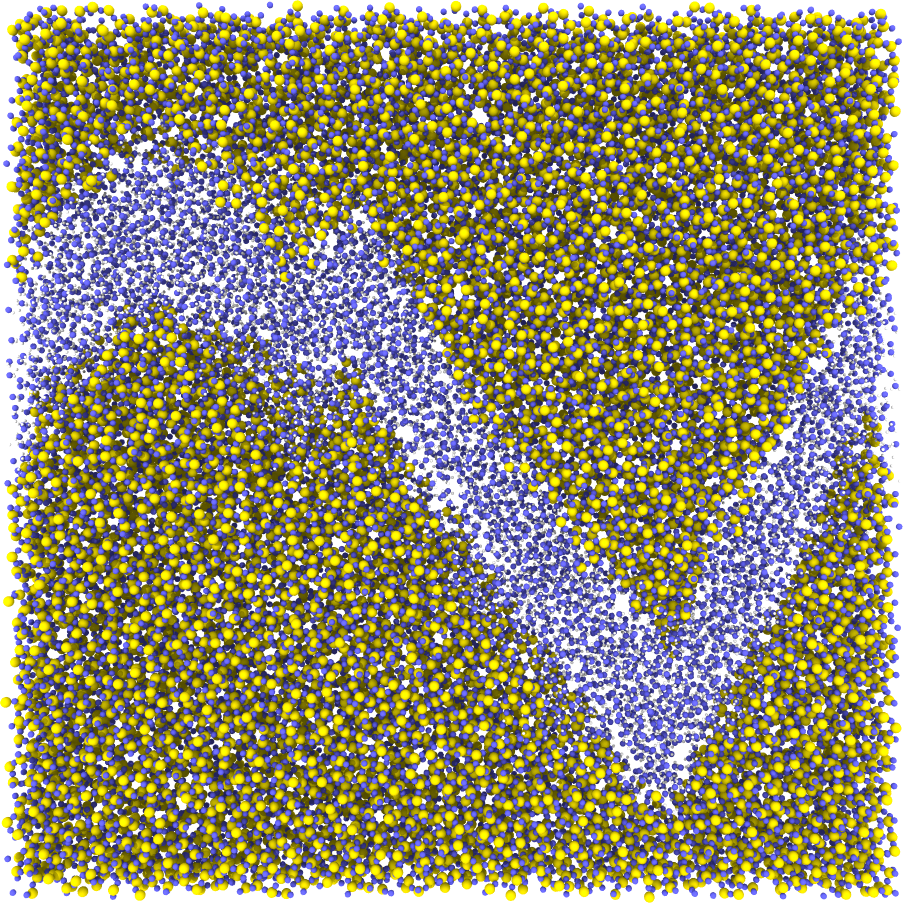
\includegraphics[width=\textwidth]{images/systems/trimmed-rough_fracture05_02_20ang}%
        \caption{20 \AA\ thick slice.}%
%         \label{fig:hex_to_tetra}%
    \end{subfigure}%
    \hfill%
    %
    % ---- Rendering just water atoms ---- %
%     \begin{subfigure}[t]{\myfigwidth}%
%         \centering% % Need to center to get image centered over caption
%         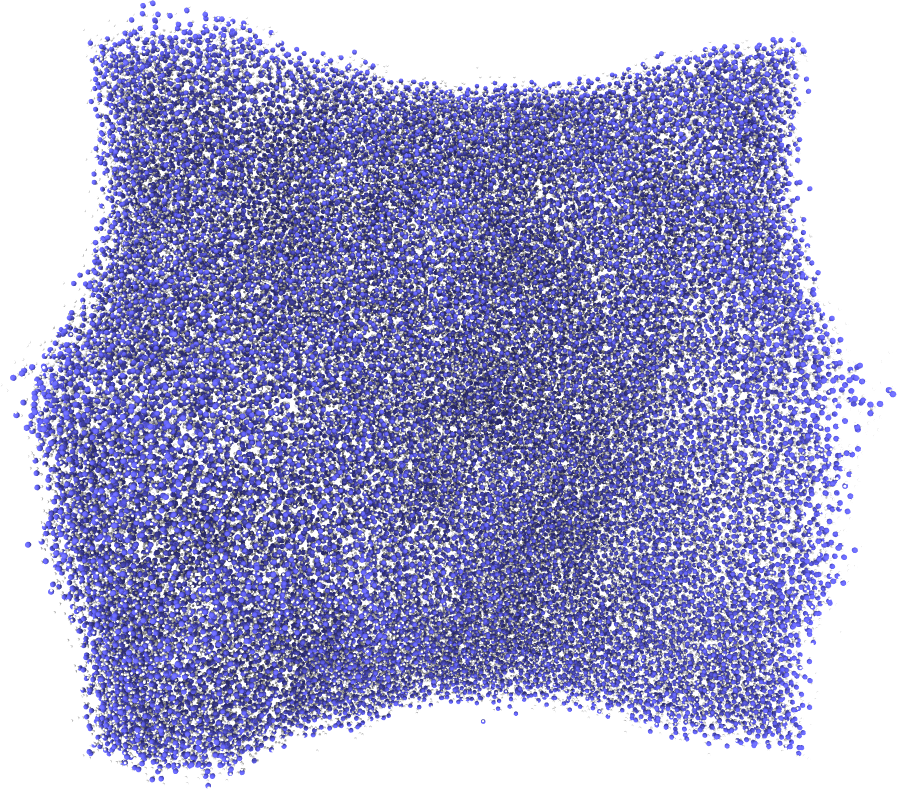
\includegraphics[width=\textwidth]{images/systems/trimmed-rough_fracture05_06}%
%         \caption{Caption.}%
% %         \label{fig:hex_to_tetra}%
%     \end{subfigure}%
    % ----
    %
    % ---- Rendering just water atoms ---- %
        \begin{subfigure}[t]{\myfigwidth}%
        \centering% % Need to center to get image centered over caption
        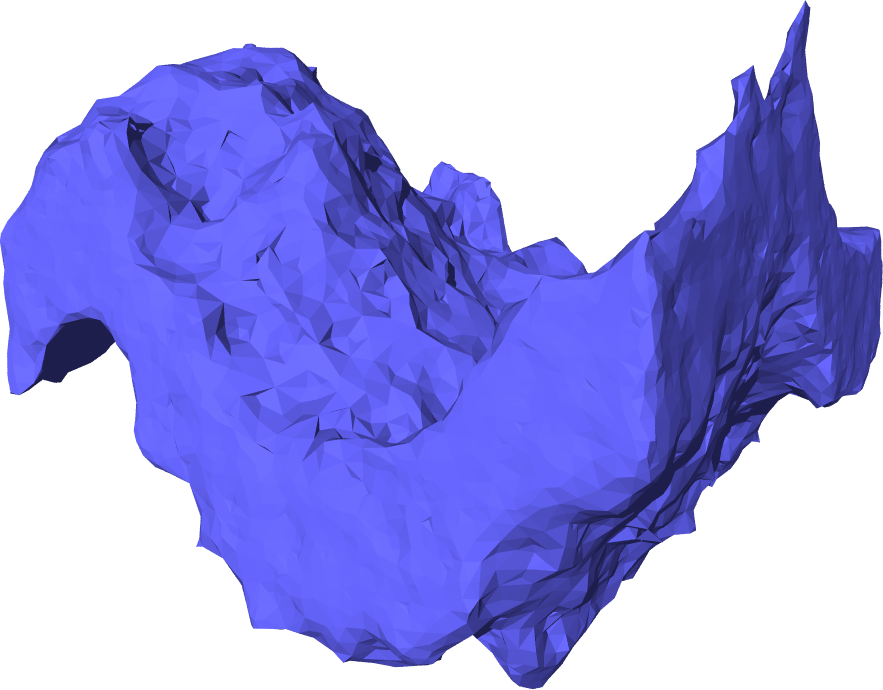
\includegraphics[width=\textwidth]{images/systems/trimmed-rough_fracture05_09}%
        \caption{The pore volume.}%
%         \label{fig:hex_to_tetra}%
    \end{subfigure}%
    % ----
    \vspace{10pt}\\%
    \caption{%
        ``Rough fracture \#4'', a randomly generated fracture generated from one surface repeated for the top and bottom half, with 28.8 \AA\ between the surfaces, giving approximately uniform width of the pore. \hl{Caption} %
        \label{fig:renderings_rough_fracture05}%
    }%
\end{figure}%

%
\begin{figure}[htpb]%
    \centering%
    \setlength{\myfigwidth}{0.49\textwidth}%
%     \setlength{\mycaptionwidth}{0.3\textwidth}%
%
    \begin{subfigure}[t]{\myfigwidth}%
        \centering% % Need to center to get image centered over caption
        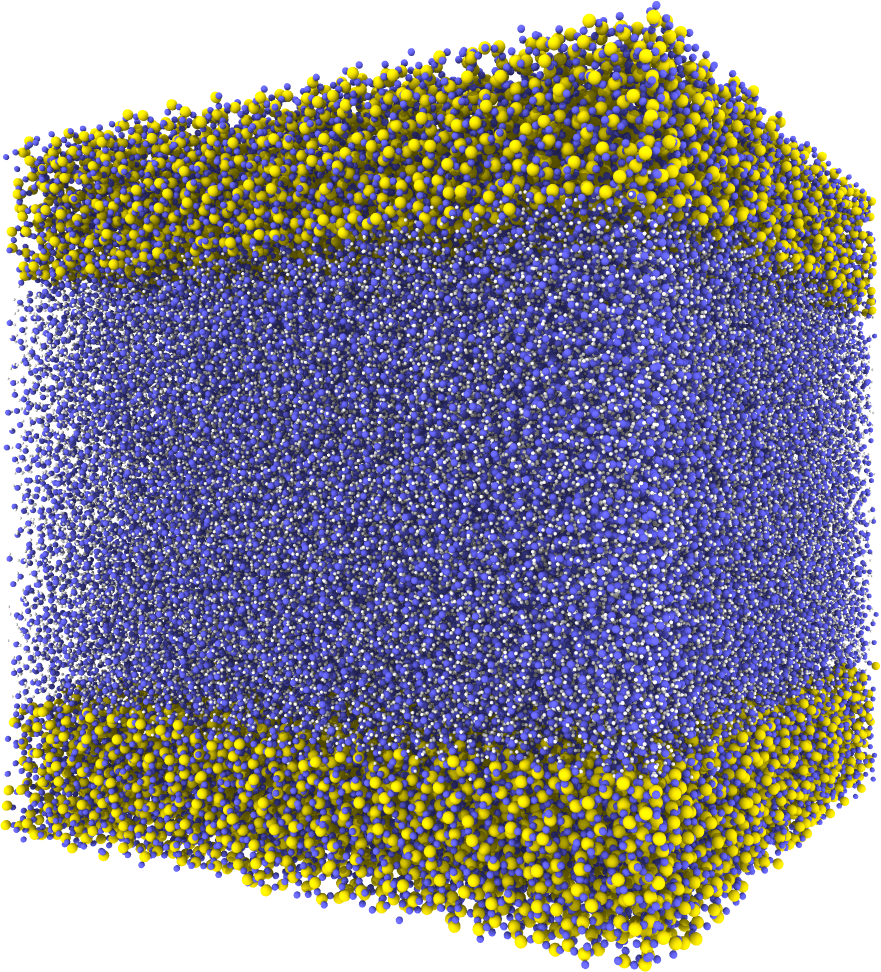
\includegraphics[width=\textwidth]{images/systems/trimmed-flat_square_fracture02_03}%
        \caption{%
            ``Reference \#1'', a 86 \AA\ wide flat pore.  \hl{Caption} %
        }%
        \label{fig:renderings_flat_square_fracture02}%
    \end{subfigure}%
    \hfill%
    \begin{subfigure}[t]{\myfigwidth}%
        \centering% % Need to center to get image centered over caption
        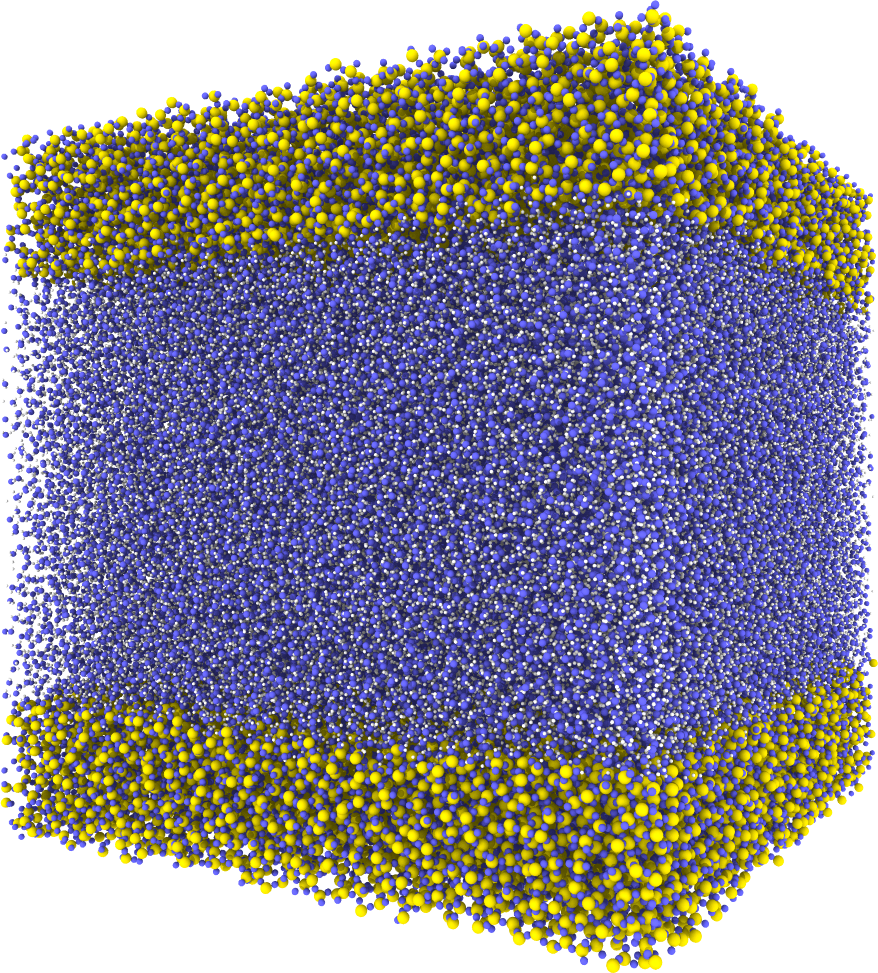
\includegraphics[width=\textwidth]{images/systems/trimmed-flat_square_fracture03_04}%
        \caption{%
            ``Reference \#2'', a 86 \AA\ wide flat pore, with higher water density than \textbf{a)}. \hl{Caption} %
        }%
        \label{fig:renderings_flat_square_fracture03}%
    \end{subfigure}%
    \vspace{10pt}\\%
    \begin{subfigure}[t]{\myfigwidth}%
        \centering% % Need to center to get image centered over caption
        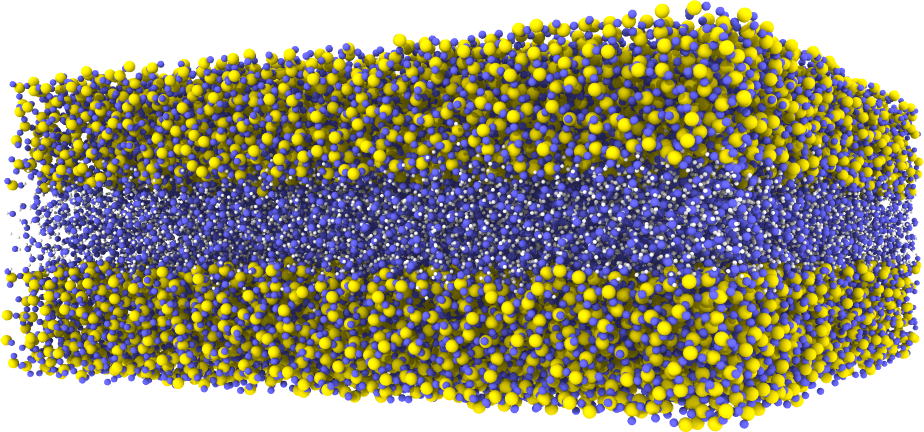
\includegraphics[width=\textwidth]{images/systems/trimmed-flat_fracture02_03}%
        \caption{%
            ``Reference \#3'', a 14.4 \AA\ wide flat pore. \hl{Caption} %
        }%
        \label{fig:renderings_flat_fracture02}%
    \end{subfigure}%
    \hfill%
    \begin{subfigure}[t]{\myfigwidth}%
        \centering% % Need to center to get image centered over caption
        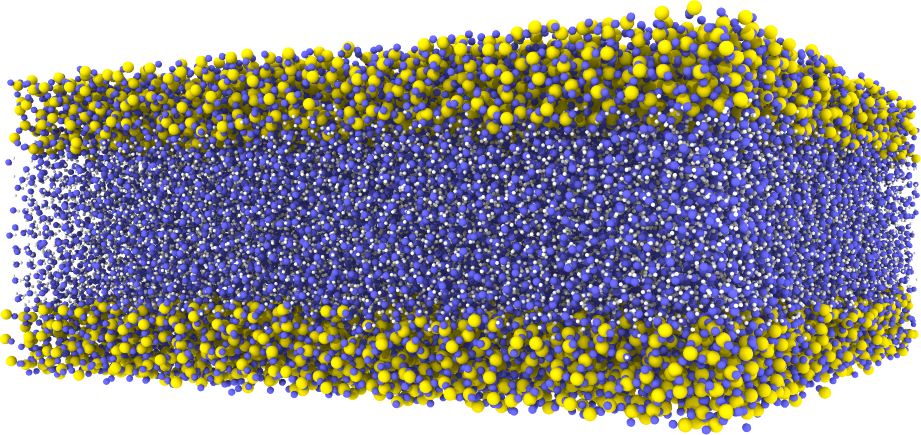
\includegraphics[width=\textwidth]{images/systems/trimmed-flat_fracture03_03}%
        \caption{%
            ``Reference \#4'', a 28.8 \AA\ wide flat pore. \hl{Caption} %
        }%
        \label{fig:renderings_flat_fracture03}%
    \end{subfigure}%
    \vspace{10pt}\\%
    \caption{%
        Reference systems \#1-4.
        \label{fig:renderings_flat_fractures}%
    }%
\end{figure}%
%